\documentclass[11pt,a4paper]{article}
\usepackage[T1]{fontenc}
\usepackage[utf8]{inputenc}
\usepackage{palatino}
\usepackage[margin=2.6cm]{geometry}
\usepackage{amsmath,amssymb}
\usepackage{booktabs}
\usepackage{graphicx}
\usepackage{longtable}
\usepackage{xcolor}
\definecolor{calteal}{HTML}{178E8E}
\definecolor{calslate}{HTML}{9AA5B1}
\usepackage[colorlinks=true,linkcolor=calteal,urlcolor=calteal,citecolor=calteal]{hyperref}
\usepackage{titlesec}
\titleformat{\section}{\normalfont\large\bfseries\color{calteal}}{\thesection}{0.7em}{}
\titleformat{\subsection}{\normalfont\normalsize\bfseries}{\thesubsection}{0.7em}{}
\usepackage{fancyhdr}
\pagestyle{fancy}\fancyhf{}
\fancyhead[L]{\small\color{calslate}emphasis --- audit and MLE-recovery study}
\fancyhead[R]{\small\color{calslate}\thepage}
\renewcommand{\headrulewidth}{0.2pt}
\usepackage{enumitem}
\setlist[itemize]{itemsep=2pt,topsep=3pt,leftmargin=1.2em}
\newcommand{\code}[1]{\texttt{\small #1}}
\newcommand{\PENDING}[1]{\par\medskip\noindent\fcolorbox{calslate}{calslate!12}{%
  \parbox{0.965\linewidth}{\small\textbf{Pending.} #1}}\par\medskip}

\title{\textbf{The \texttt{emphasis} diversification estimator:\\
audit, repair, and recovery of the maximum-likelihood estimate}}
\author{Francisco Richter\\\small Università della Svizzera italiana}
\date{\today}

\begin{document}
\maketitle

\begin{abstract}
\noindent
\code{emphasis} estimates the parameters of a birth--death diversification process from a
reconstructed phylogeny without evaluating the marginal likelihood directly. It augments the
observed tree with the lineages that went extinct or were not sampled, weights each augmented
tree by importance sampling, maximises the weighted complete-data log-likelihood, and iterates:
Monte Carlo EM. A cross-entropy search supplies the starting point. This report documents three
things: what the implementation computes, which of its components were found to be incorrect and
what was changed, and how closely the resulting estimator reaches the exact maximum-likelihood
estimate on trees where that estimate can be computed in closed form.
\end{abstract}

\section{Scope and method}

The work had three stages, each carried out by a set of independent agents whose findings were
verified against a closed form, a property, or a controlled comparison before being recorded.

\begin{enumerate}[leftmargin=1.4em]
\item \textbf{Reading.} Seven readers mapped one subsystem each and wrote out the quantities the
  code computes, with file and line anchors: the proposal densities, the importance weights, the
  estimator $\widehat{f}$ of the marginal log-likelihood, the M-step objective, and the index,
  time, and log conventions. The result is \code{dev/audit/01-map.md}. Each reader also recorded
  the points at which the code might not compute what the surrounding documentation claims. These
  became 105 numbered hypotheses.
\item \textbf{Testing.} Every hypothesis rated critical or major was given to a verifier, which
  had to produce a runnable reproduction, and then to an independent replicator, which was asked
  to refute it. Lower-severity hypotheses were triaged in themed batches. Reproduction scripts are
  in \code{dev/audit/checks/}; the outcome of each is in \code{dev/audit/02-findings.md}.
\item \textbf{Repair and measurement.} The findings that change the numbers a constant-rates or
  diversity-dependent fit returns were implemented, reviewed adversarially, and merged. The
  estimator was then measured against exact references.
\end{enumerate}

\section{The estimator as implemented}

Let $y$ be the branching times of the reconstructed tree and $z$ an augmentation of it with
unobserved lineages. The marginal likelihood integrates over the augmentations,
\[
  L_\theta(y) \;=\; \int f_\theta(y, z)\,\mathrm{d}z ,
\]
and is estimated by importance sampling from a proposal $q$: with draws $z_1,\dots,z_S$,
\[
  \widehat{f} \;=\; \log\Big( \tfrac{1}{S}\textstyle\sum_i \exp(\log f_\theta(y,z_i) - \log q(z_i)) \Big).
\]
The M-step maximises $Q(\theta) = \sum_i w_i \log f_\theta(y, z_i)$ over the weights of the current
E-step, and the two steps alternate to convergence.

Two proposals exist. The \textbf{BDI} sampler draws from the exact conditional distribution of the
missing lineages under constant rates, which makes the weights constant and $\widehat{f}$ exact up
to Monte Carlo error of zero; under diversity dependence it solves a mean-field backward--forward
system and its draws are rejected when they leave survivors at the present. The \textbf{thinning}
sampler proposes events by Poisson thinning under a dominating rate envelope and covers every
model and link. Section~\ref{sec:results} reports what each achieves.

\subsection{Conventions that the report depends on}
\begin{itemize}
\item Branching times are passed crown-age first, in decreasing order; the crown is two lineages
  at forward time zero.
\item $f$ is a per-lineage labelled density: it carries no multiplicity factors. Measured against
  \code{DDD::bd\_loglik} with \code{btorph = 1}, the constant between the two is zero, so
  log-likelihood \emph{differences} and \emph{maximisers} are directly comparable.
\item The default fit is unconditioned (\code{cond = NULL}), which targets
  \code{DDD::bd\_ML(cond = 0, soc = 2)}. The conditioned fit targets
  \code{bd\_ML(cond = 1)}, which equals \code{ape::birthdeath}.
\end{itemize}

\section{Audit outcome}

Of the 105 hypotheses, 94 were confirmed and 11 were refuted; of the confirmed, 89 are defects
and 5 are design decisions that only the author can settle. Figure~\ref{fig:audit} gives the
distribution by subsystem.

\begin{figure}[h]\centering
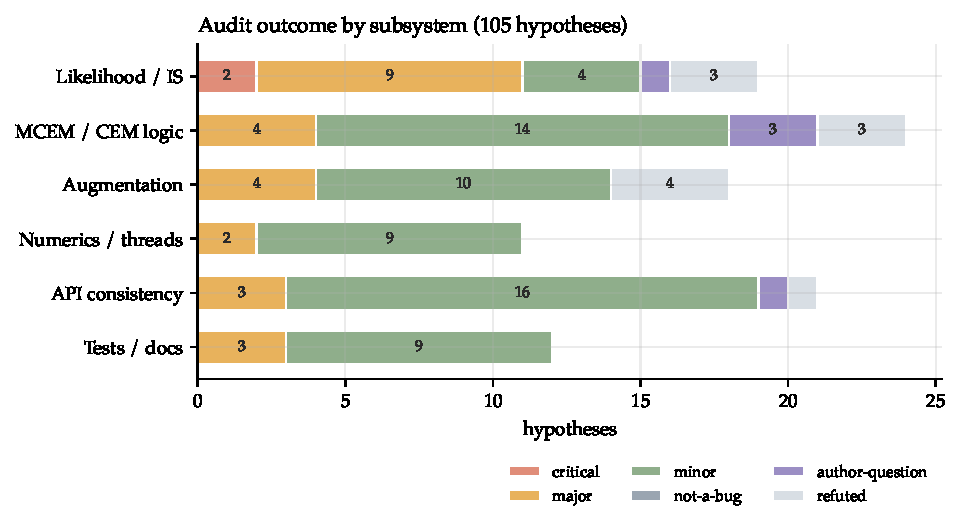
\includegraphics[width=\linewidth]{figures/fig1-audit-outcomes.pdf}
\caption{Outcome of every hypothesis, by subsystem. A hypothesis counts as refuted when either the
verifier or the independent replicator refuted it; the severity shown is the replicator's, not the
one originally proposed.}
\label{fig:audit}
\end{figure}

\subsection{Findings that changed the numbers}

\begin{itemize}
\item \textbf{A zero rate produced $+\infty$ rather than $-\infty$.} In the accumulator that forms
  the speciation term of $\log f$, the sign of a non-finite result was taken from a running sum, so
  an augmented tree containing a lineage with zero speciation rate could be assigned infinite
  positive log-density. Under a diversity-dependent model on the linear link such trees arise
  whenever the augmented richness reaches the zero of $\lambda(N)$.
\item \textbf{The exact sampler could not enter the high-turnover region.} For $\mu_0 \ge \lambda_0$
  a sign test in the closed-form integral returned $+\infty$ for every segment, so every draw
  failed. Measured before the change: 0 of 8 draws finite; after: 8 of 8.
\item \textbf{The survival penalty was diluted.} With a conditional supplied, the M-step added
  $\log P_\theta(\text{survival})$ to a weighted sum whose weights were unnormalised, so the
  penalty entered with relative strength $1/\sum_i w_i$ and the conditioned fit returned close to
  the unconditioned maximiser.
\item \textbf{The BDI estimator of $\widehat{f}$ omitted its rejection term.} Under diversity
  dependence the sampler rejects draws that leave survivors, so it estimates
  $\log L - \log P(\text{accept})$. Regressing the gap on $-\log(\text{acceptance})$ gave slope
  1.006 with $R^2 = 0.964$.
\item \textbf{The stopping rule depended on the unit of time.} Convergence was declared on a
  parameter change scaled by the user's bound box. Replacing the box by a floor that carries the
  parameter's units makes the statistic invariant: the same tree with branching times multiplied
  by $10^3$ now takes the same path and stops for the same reason.
\item \textbf{The thinning envelope did not dominate.} Acceptance probabilities exceeded one on
  roughly half the candidates of a test tree, so the sampler drew fewer missing lineages than its
  own density charged. The envelope now uses the post-event lineage count.
\end{itemize}

\subsection{Findings outside the numbers}

Two are worth stating because they affect anyone who installs the package rather than only the
estimates it returns.

\begin{itemize}
\item \textbf{The package did not build against a current \code{RcppParallel}.} It used
  \code{tbb::task\_scheduler\_init}, removed in oneTBB, and compiled only because
  \code{RcppParallel} 5.1.11.2 still ships the legacy header.
\item \textbf{\code{num\_threads} did not bind.} Both parallel regions constructed a task arena and
  then ran the parallel algorithm outside it, so the work executed on the default arena, sized by
  hardware concurrency (Figure~\ref{fig:threads}).
\end{itemize}

\begin{figure}[h]\centering
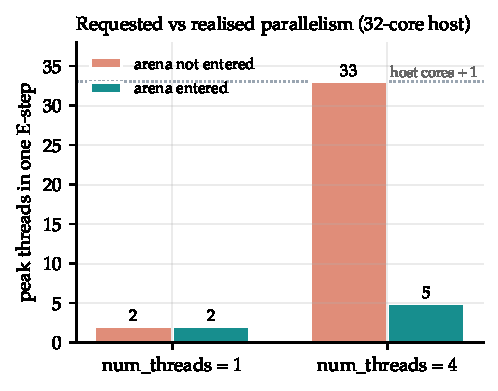
\includegraphics[width=0.52\linewidth]{figures/fig2-thread-binding.pdf}
\caption{Peak threads in one E-step on a 32-core host, before and after the parallel region was
moved inside the arena. A request for four threads was served by the whole machine.}
\label{fig:threads}
\end{figure}

\section{The validation study}

\subsection{Question and estimand}

The question is how closely the estimator reaches the \emph{exact maximum-likelihood estimate of
the tree in hand}, not how closely it recovers the parameters that generated the tree. The two
differ by the sampling error of the MLE itself, which is a property of the data and not of the
method. The primary scalar is therefore the log-likelihood deficit
\[
  \Delta\ell \;=\; \ell_{\text{exact}}(\widehat{\theta}_{\text{emphasis}})
                 - \ell_{\text{exact}}(\widehat{\theta}_{\text{MLE}}) \;\le\; 0 ,
\]
which is free of the parameterisation, defined when the MLE sits on the boundary $\mu = 0$, and
has a natural scale: $0.5$ nats is about one standard error in one parameter. Recovery of the
generating parameters is reported beside it, never mixed into it.

\subsection{Design}

Trees are simulated over a grid of tree size $n$ and turnover $\varepsilon = \mu/\lambda$ for the
constant-rates arm, and in three diversity-dependent regimes. Each tree is fitted from a start far
from the optimum and again from the exact MLE --- the first measures the search, the second the
refinement alone --- with both samplers, at three Monte Carlo sample sizes, with replicate fits so
that Monte Carlo scatter can be separated from systematic displacement. A fixed-$\theta$ arm
compares $\widehat{f}$ with the exact log-likelihood on a grid around the MLE, which separates bias
in the weights from variance in them. Exact references are \code{DDD::bd\_ML} for constant rates
and \code{DDD::dd\_ML} for the linear diversity-dependent model; the calls, their conditioning
flags, and the parameter mapping are in \code{dev/validation/00-design.md}.

Decision rules were fixed before the main tier ran. Every fit is recorded with an outcome and none
is excluded, so a configuration that exhausts its budget appears as a coverage statistic rather
than silently improving the cells that finished.

\subsection{Reference gate}

Seven identities and three build sentinels are asserted before any fit runs. All pass on the
repaired build. The identities establish that the exact references agree with each other and with
the closed form to $10^{-4}$ or better, and that the package's own $\widehat{f}$ reproduces the
closed-form likelihood to $1.6\times10^{-11}$ with weights of zero variance. The sentinels
establish that the three repairs above are present in the build being measured.

\section{Results}\label{sec:results}

\PENDING{The main tier is running: 2431 fits over the constant-rates grid, the three
diversity-dependent regimes, the fixed-$\theta$ surface, and the full pipeline. This section will
report, per cell: the distribution of $\Delta\ell$ decomposed into Monte Carlo scatter and
systematic displacement, the bias of each parameter in units of its standard error, the accuracy
of the reported log-likelihood, the effective sample size of the importance weights, the fraction
of fits that converge, and the verdict of each cell against the pre-registered decision rules.}

\section{Discussion}

\PENDING{To be written from the results: which regimes the estimator covers, which it does not,
what the remaining loss is attributable to, and what would have to change for the uncovered
regimes. The audit's waves~2 and~3 are not applied, and the items in them that bear on the answer
are named here.}

\section{Reproduction}

Everything in this report is regenerated from the repository. The audit's reproduction scripts are
in \code{dev/audit/checks/}; the study runs through \code{dev/validation/run.sh}, which gates on
the reference identities, simulates, computes the exact references, fits, and analyses, in tiers.
Each result row carries a fingerprint of the build that produced it, and the driver refuses to mix
builds within one results directory.

\end{document}
